\documentclass{beamer}

\setbeamertemplate{caption}[numbered]
\usetheme{Hannover}
\usepackage{subcaption}

\begin{document}

\title{Firefly: Exploiting Implicit Trust in Satellite Downlink Processing Systems}
\author[Edd Salkield]{
  \emph{Edd Salkield}
  \inst{1}
  \and
  Joshua Smailes
  \inst{1}
  \and
  Richard Baker
  \inst{1}
  \and
  Martin Strohmeier
  \inst{2}
  \and
  Ivan Martinovic
  \inst{1}
}
\institute[University of Oxford]{
  \inst{1} Systems Security Lab, University of Oxford \and %
  \inst{2} Cyber-Defence Campus, armasuisse Science + Technology
}
\date{Trinity 2022}

\begin{frame}
  \titlepage
\end{frame}

% other opening: shattering expectations on use of crypto to secure the downlinks


%\begin{frame}
%  \frametitle{What's new in space?}
%  \begin{itemize}
%    \item New space applications
%    \item Some graph showing forecast growth
%  \end{itemize}
%  \note{New space is the new thing}
%\end{frame}
% Satellite data has never been more important, and we've seen ongoing commercialisation of the space industry

\begin{frame}
  \frametitle{What's new in space?}
  \framesubtitle{Commercially competitive launch providers}
  Existing national launch providers being challenged with lower costs through space startups
  
  \begin{columns}[t]

    \begin{column}{5cm}
      \begin{figure}
        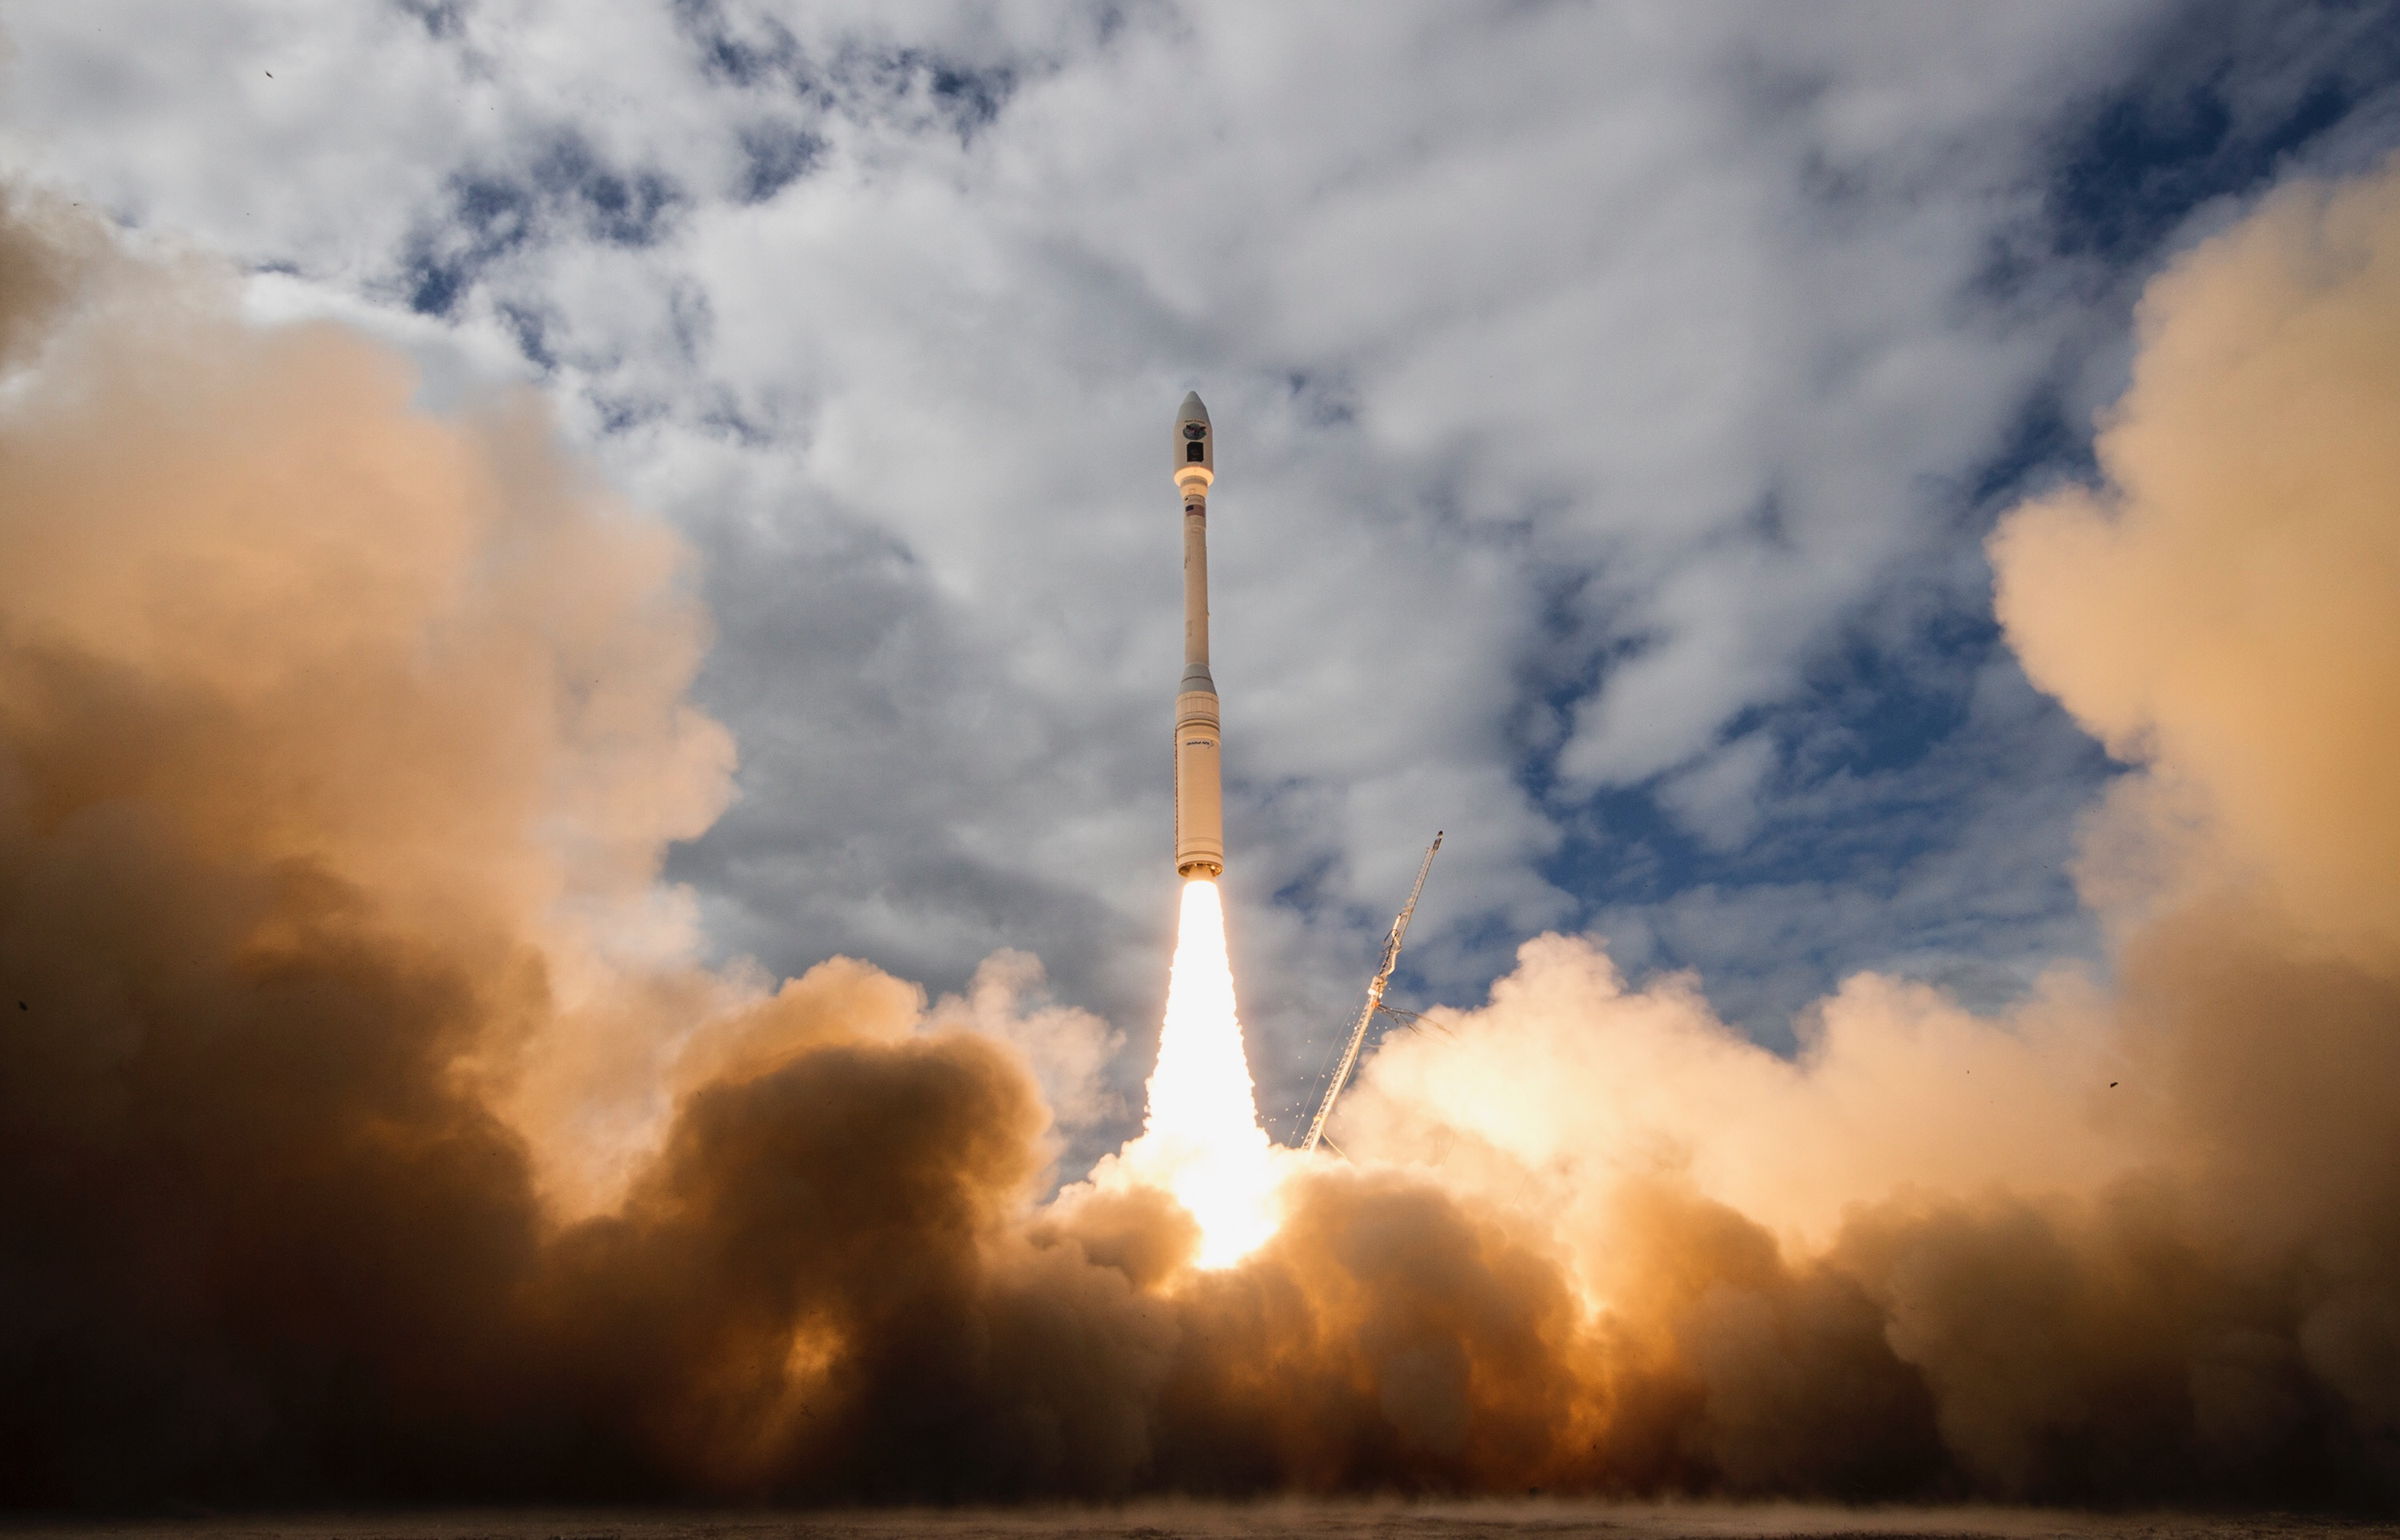
\includegraphics[width=0.8\textwidth]{images/planetlabs_launch.jpg}
        \caption{Launch of SkySats 8-13 and Flock 3m, Image: Orbital ATK}
        \label{fig:space_segment}
      \end{figure}
    \end{column}

    \begin{column}{5cm}
      \begin{figure}
        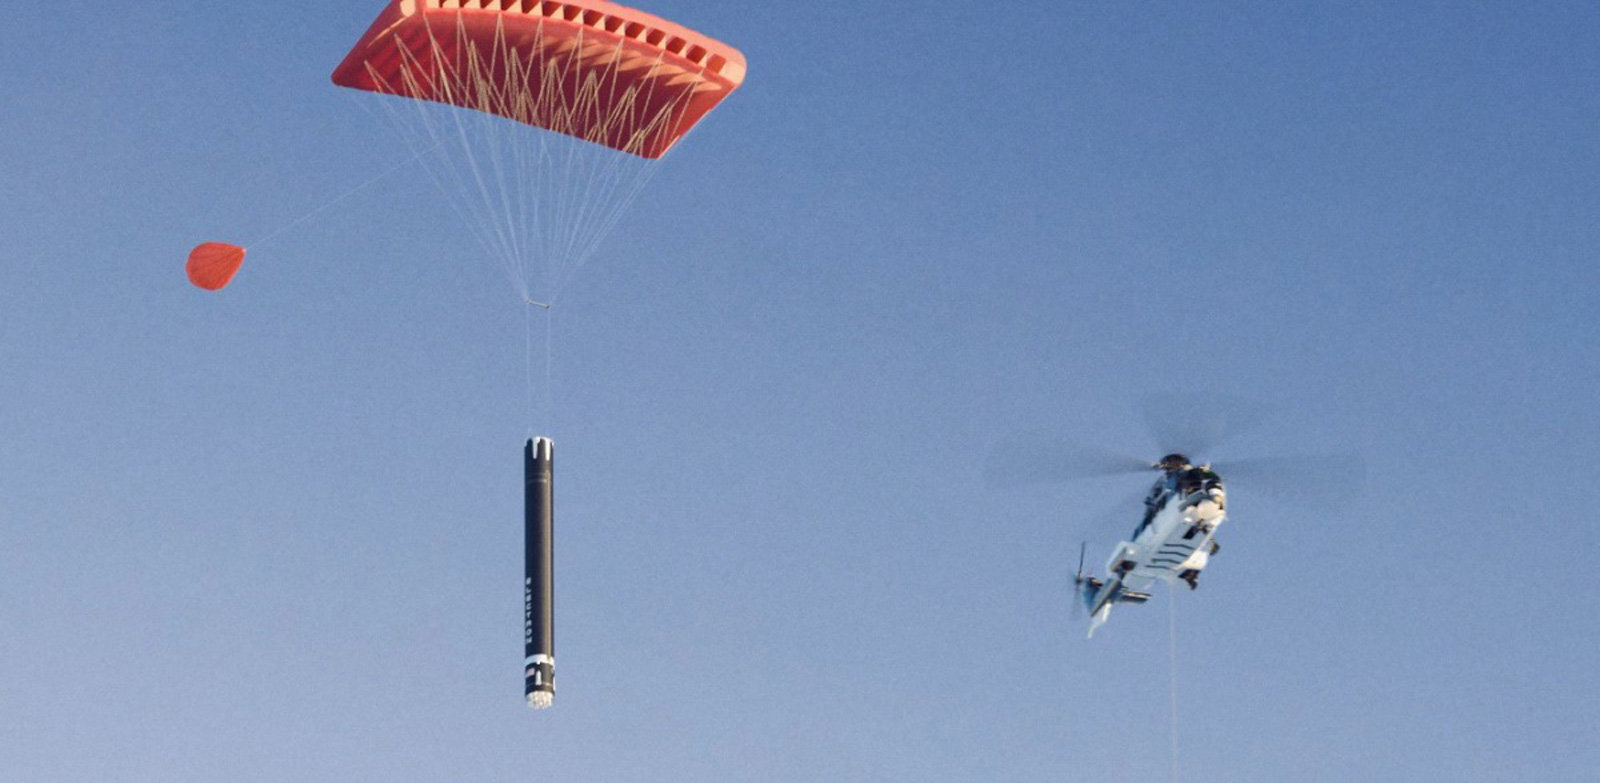
\includegraphics[width=0.8\textwidth]{images/rocket_lab_capture.jpeg}
        \caption{In-air helicopter Rocket Labs capture, Image: Rocket Labs}
        \label{fig:space_segment}
      \end{figure}
    \end{column}

  \end{columns}
\end{frame}

\begin{frame}
  \frametitle{What's new in space?}
  \framesubtitle{Constellations for internet routing}
  \begin{figure}
      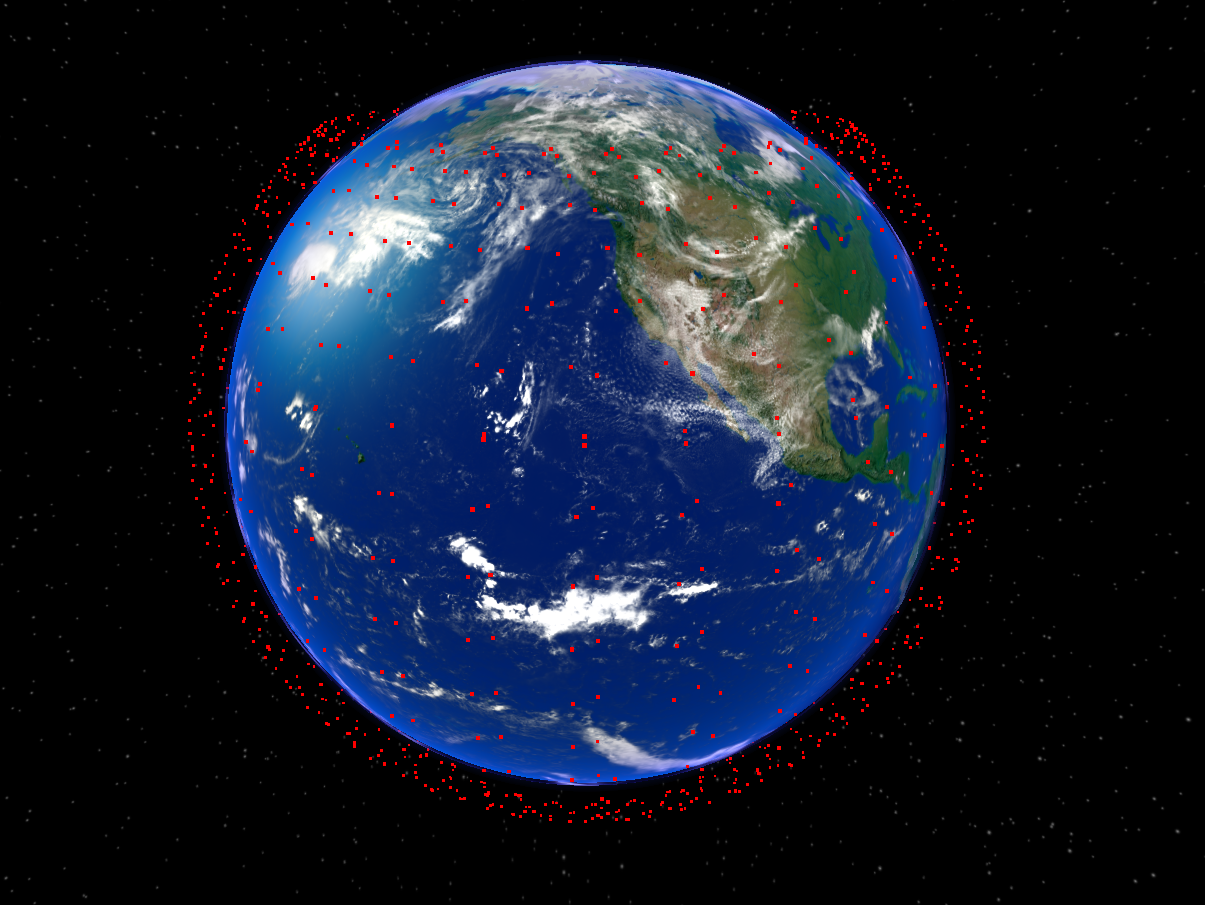
\includegraphics[width=0.8\textwidth]{images/starlink_current.png}
      \caption{Current starlink deployment}
      \label{fig:space_segment}
  \end{figure}
  \textit{Death by a Thousand COTS, Frederick Rawlins}~\cite{rawlins2022death}
\end{frame}

\begin{frame}
  \frametitle{What's new in space?}
  \framesubtitle{Constellations for internet routing}
  \begin{itemize}
    \item SpaceX Starlink
    \item OneWeb
    \item Kuiper
  \end{itemize}
\end{frame}

\begin{frame}
  \frametitle{What's new in space?}
  \framesubtitle{New Earth-observing capabilities}

  \begin{columns}[t]

    \begin{column}{5cm}
      \begin{figure}
        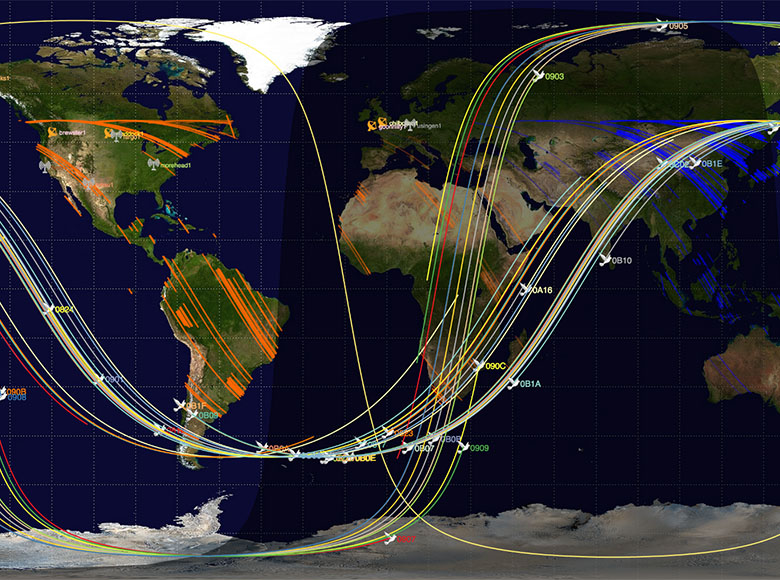
\includegraphics[width=0.8\textwidth]{images/planetlabs_orbit_operations.jpg}
        \caption{Planet Labs constellation map, Image: Planet}
        \label{fig:space_segment}
      \end{figure}
    \end{column}

    \begin{column}{5cm}
      \begin{figure}
        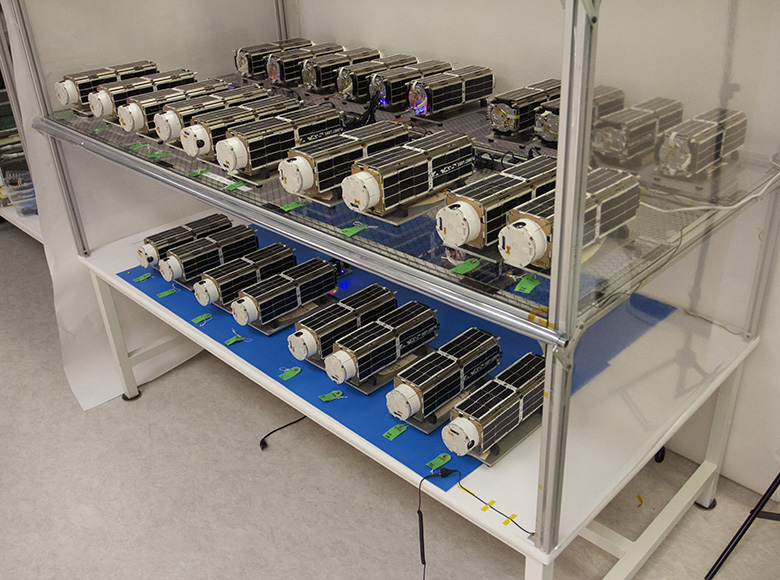
\includegraphics[width=0.8\textwidth]{images/planetlabs_satellites.jpg}
        \caption{Rack of Planet Lab ``Dove" satellites, Image: Planet}
        \label{fig:space_segment}
      \end{figure}
    \end{column}
  \end{columns}
  \note[item]{So are we starting to learn from our mistakes? Yes!}
\end{frame}

\begin{frame}
  \frametitle{Security benefits of new space}
  \begin{itemize}
    \item Standardisation of (encrypted) network protocols
    \item Use of well-understood hardware, similar to terrestrial systems
    \item Security-critical OS components open sourced and auditable
    \item More attention on considering security throughout the design process
  \end{itemize}

  \onslide<2>
  Thankfully these new space satellites supercede the old and insecure ones, so the old ones have just gone away right?
  \note{
    In comparison, many of the satellites designed years ago weren't designed with security in mind, because they didn't need to.
    Interfacing with the satellite over the radio link would require an incredibly expensive and specialised setup that only nation states could realistically pull attacks off.

  Thankfully these new space satellites supercede the previous ones, so the old ones have just gone away right?
  }
\end{frame}

\begin{frame}
  \frametitle{Unencrypted satellite communications}

  \begin{figure}
      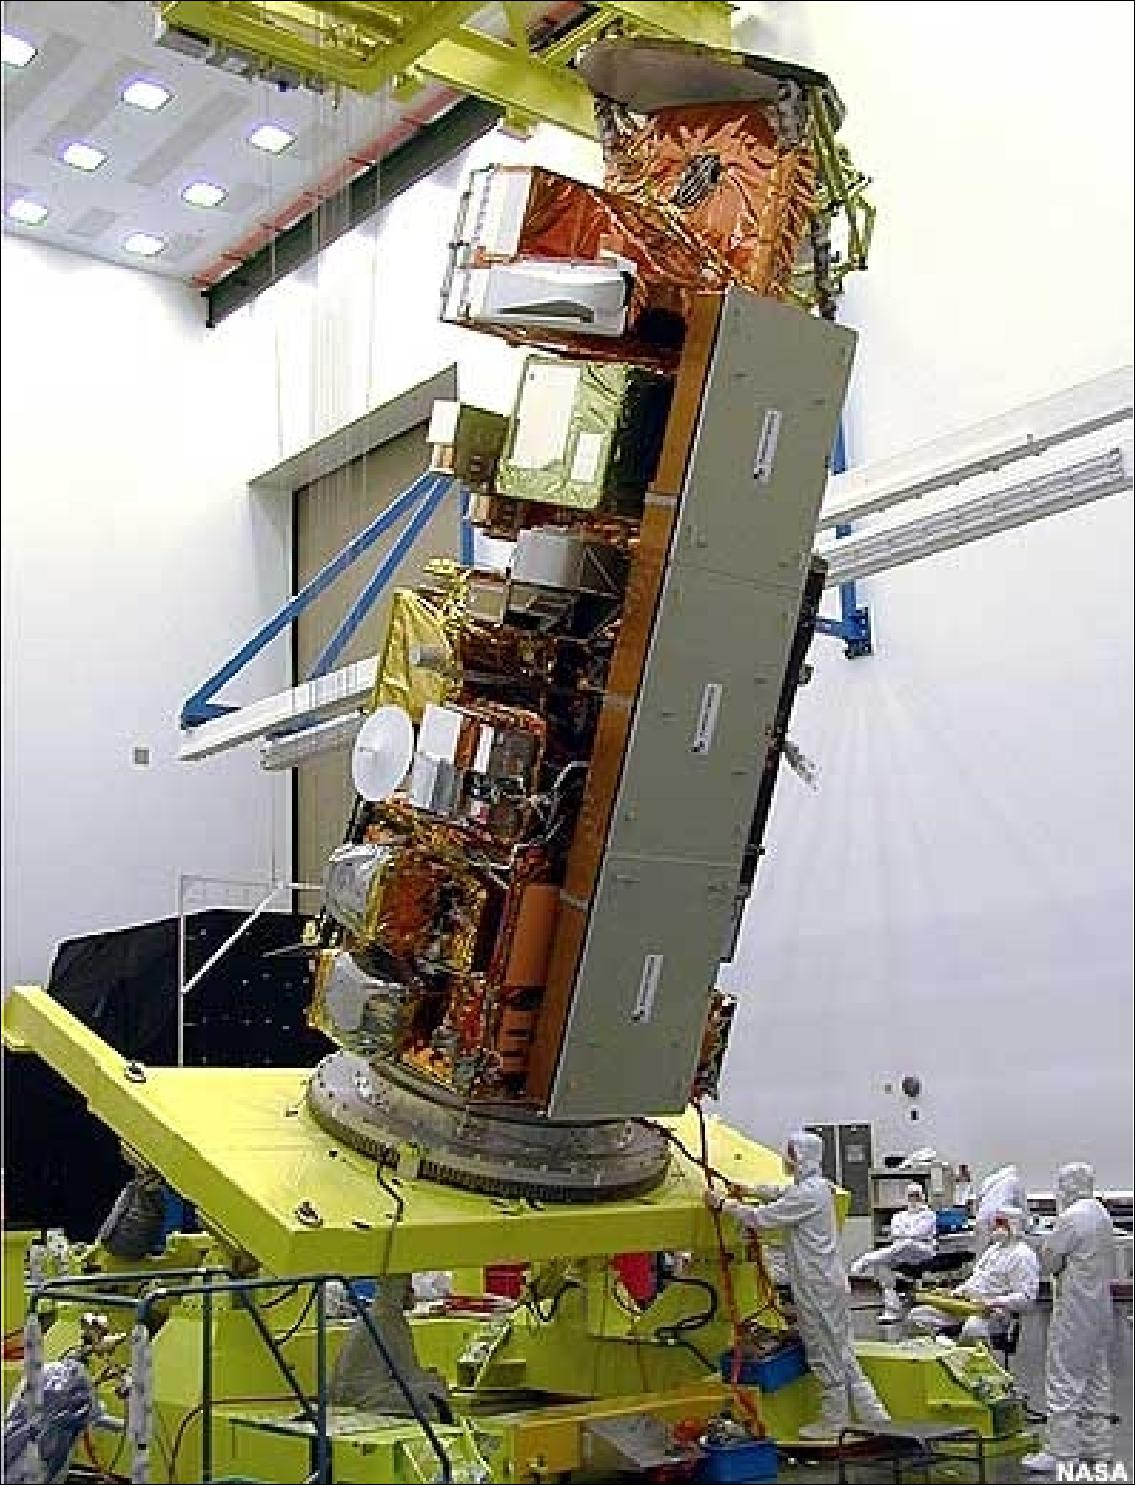
\includegraphics[width=0.4\textwidth]{images/aqua.jpeg}
      \caption{Aqua: part of NASA's Earth Observing Satellite fleet launched in 2002}
      \label{fig:aqua}
  \end{figure}

  \onslide<2>
  Well okay, but at least nobody uses them for anything...

  \note{
    essentially orbiting research stations - cutting edge at launch with many onboard instruments
    not obsoleted, since highly specialised
    still producing highly useful sensor data today
    we wouldn't want to replace them, even if we could, due to the cost
  }
\end{frame}

\begin{frame}
  \frametitle{Forest fire detection}
  \begin{figure}
      \centering
      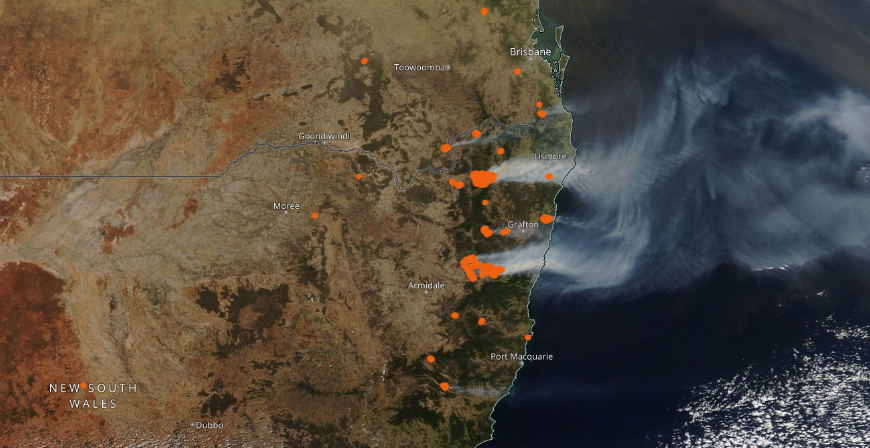
\includegraphics[width=\columnwidth]{images/bushfire.png}
      \caption{The 2019 Australia bushfires as seen from Aqua's MODIS instrument, annotated with the \textit{Fires and Thermal Anomalies} dataset on NASA's worldview.\protect\footnotemark}
      \label{fig:bushfire}
  \end{figure}

  \onslide<2>
  Well okay, but at least people are aware that the data sources are unauthenticated right?
\end{frame}

\begin{frame}
  \frametitle{Forest fire detection}
  \begin{figure}
      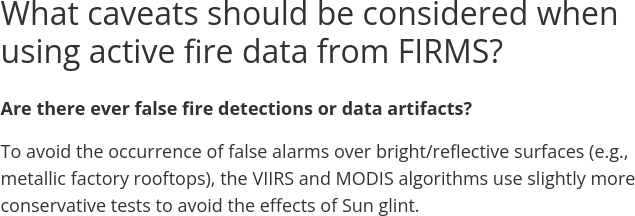
\includegraphics[width=\columnwidth]{images/firms_faq.png}
      \caption{Excerpt from the FIRMS FAQ \url{https://www.earthdata.nasa.gov/faq/firms-faq\#ed-false-detections}}
      \label{fig:bushfire}
  \end{figure}

  \onslide<2>
  Well okay, but at least some of these old satellites do implement cryptographic authenticity checks...
\end{frame}



% TODO: maybe insert slides with fire pictures

\begin{frame}
  \frametitle{Weak cryptographic implementations}
  \begin{columns}[t]
    \begin{column}{4cm}
      \begin{figure}
          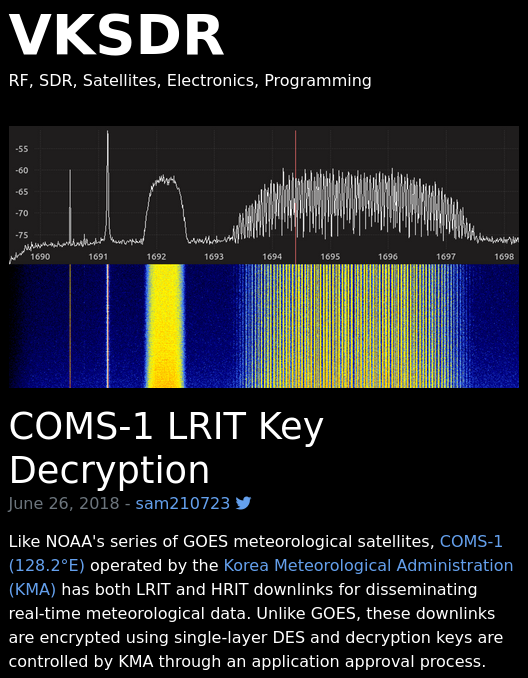
\includegraphics[width=\columnwidth]{images/lrit-key-dec.png}
          \label{fig:lrit-key-dec}
      \end{figure}
    \end{column}

    \begin{column}{4cm}
      \begin{figure}
          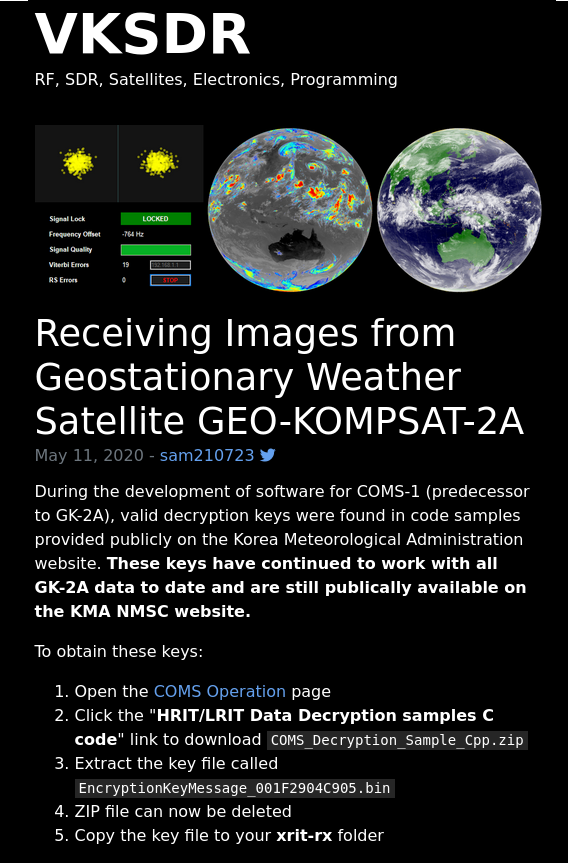
\includegraphics[width=\columnwidth]{images/xrit-rx.png}
          \label{fig:xrit-rx}
      \end{figure}
    \end{column}

  \end{columns}
  \url{https://vksdr.com/}
  \note{
    Explain how a combination of weak crypto (DES 1), hardcoded keys, and and bad key management has lead to these Korean satellites being essentially unencrypted
    It's hard to blame anyone - the threat landscape has shifted so much
    crypto has come along a long way, and these satellites are up for decades or more
  }
\end{frame}

\begin{frame}
  \frametitle{What's old in space?}
  \begin{itemize}
    \item Legacy satellite systems currently exist, which either do not implement cryptographic authenticity guarantees at all, or do so weakly
    \item These satellites were cutting edge at their launch, and still produce highly valuable scientific data
    \item Derived datasets are used widely, including for critical national infrastructure
    \item The hardware generally isn't powerful enough to implement crypto in software
    \item Retrofitting cryptographic modules is impractical and highly expensive
  \end{itemize}
\end{frame}

\begin{frame}
  \frametitle{Current situation}
  \begin{itemize}[<+->]
    \item Most current work focusses on new space, proposing countermeasures against known attack classes
    \item However, advances in hardware and attack techniques are making whole classes of existing satellites vulnerable
    \item Since the advent of the software-defined radio, mounting an injection attack against an insecure satellite downlink requires only access to off-the-shelf hardware
    \item There's no current research investigating the impact of a modern adversary overshadowing Earth monitoring satellites
  \end{itemize}
  \note{
    In order to investigate the effect of an attacker against such a system, we first have to understand how the system works.
  }
\end{frame}

% TODO: expand out into slides with images instead
\begin{frame}
  \frametitle{Satellite-derived datasets}
  Satellite data is a key part of national, personal, and scientific infrastructure.
  \newline

  Earth monitoring satellite data is often used in cases such as:

  \begin{itemize}
    \item Forest fire detection
    \item Analysis of activities in conflict areas
    \item Environmental monitoring
  \end{itemize}
  \note{So how are these datasets produced?}
\end{frame}

% TODO: simplify diagram
\begin{frame}
  \frametitle{Satellite downlink communications}
  \begin{figure}
      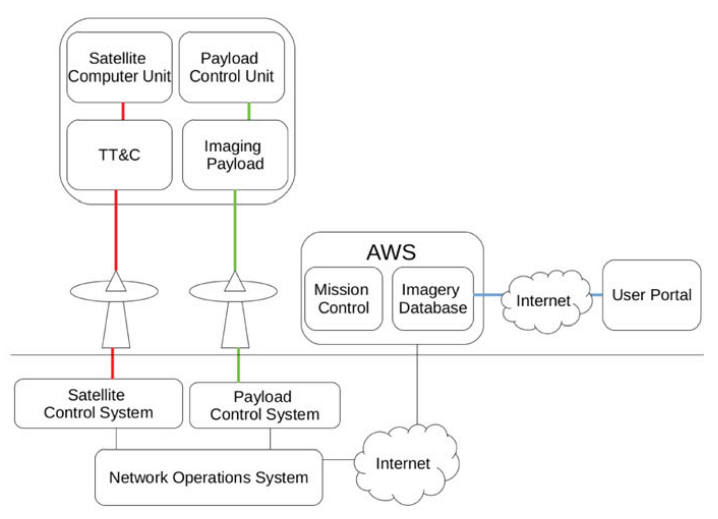
\includegraphics[width=0.65\textwidth]{images/dataset_generation.png}
      \caption{Ground segment architecture for web-based access}
      \label{fig:space_segment}
  \end{figure}

  If an attacker can control the communications, they can affect the derived datasets
\end{frame}
% From satellite, through some processing system, and then out via the internet
% Now of course, if a satellite implements good cryptographic authenticity, then an attacker can only deny service through jamming the physical layer. However against an unencrypted satellite downlink, the attacker can potentially affect the communications in much more subtle ways.

\begin{frame}
  \frametitle{Forest fire detection}
  \begin{figure}
      \centering
      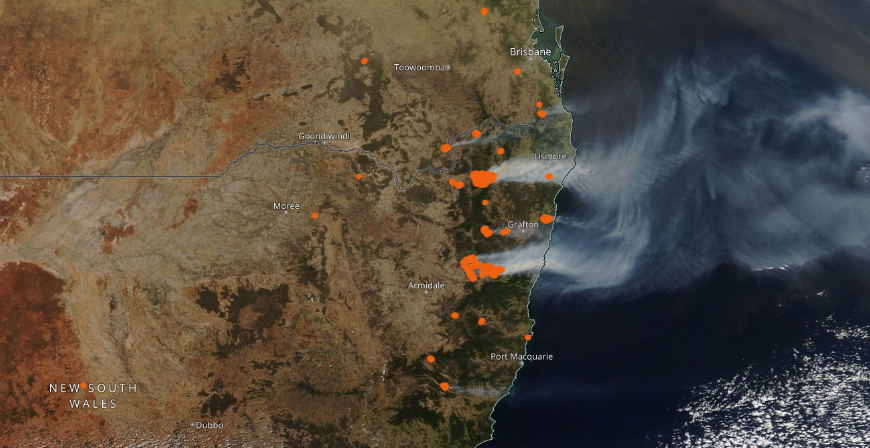
\includegraphics[width=\columnwidth]{images/bushfire.png}
      \caption{The 2019 Australia bushfires as seen from Aqua's MODIS instrument, annotated with the \textit{Fires and Thermal Anomalies} dataset on NASA's worldview.\protect\footnotemark}
      \label{fig:bushfire}
  \end{figure}
\end{frame}
% Taking forest fire detection as a case study, through injecting a custom signal, an attacker may be able to affect where and how fires are detected
% This sensor data is used to produce derived datasets like FIRMS
% Open up FIRMS map to demo scrolling around various images
% Explain how nation state departments use this API
% If an attacker can successfully inject data, they could manipulate this service to trigger false emergency response or mislead crisis analysis
% So how might an attacker inject data like this?

% TODO: too much text
\begin{frame}
  \frametitle{Overshadowing the physical layer}
  \begin{figure}
      \centering
      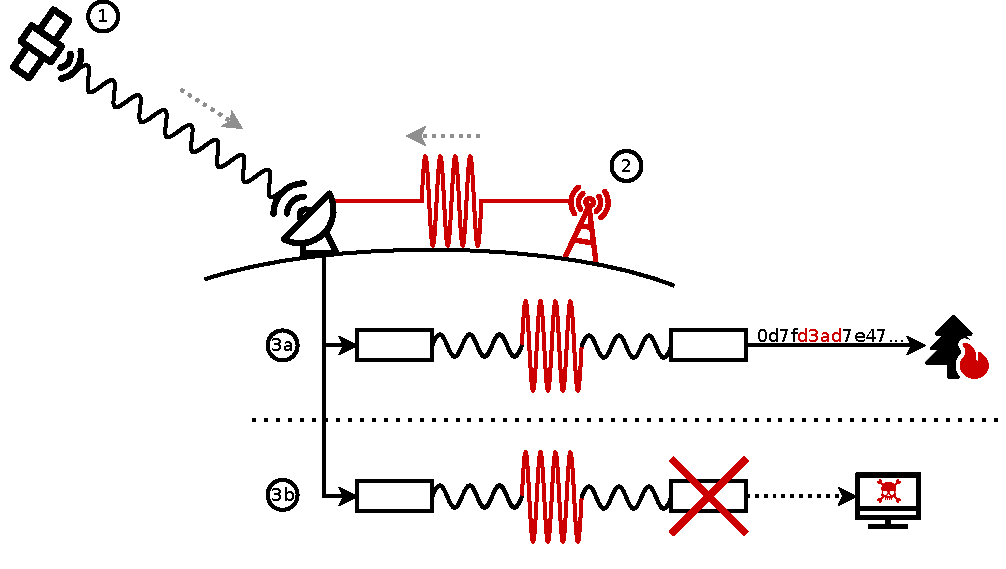
\includegraphics[width=0.7\textwidth]{images/attack_illustration.pdf}
      \caption{1)~The satellite broadcasts a signal; 2)~A ground-based attacker injects a crafted signal, overshadowing the legitimate signal and resulting in one of two scenarios; 3a)~The victim receiver decodes the attacker-controlled data, poisoning derived datasets; 3b)~The injected signal exploits vulnerabilities in the protocol decoders.}
      \label{fig:attack-illustration}
  \end{figure}
\end{frame}
% In this work, we consider the physical layer
% A number of challenges relating to the physical layer include:
% * Ground-based attacker against a highly directional dish
% * Generating the correct data
% * Timing it agaist the original signal

\begin{frame}
  \frametitle{Forest fire detection}
  \framesubtitle{Injecting ficticious fires}

  \begin{figure}
    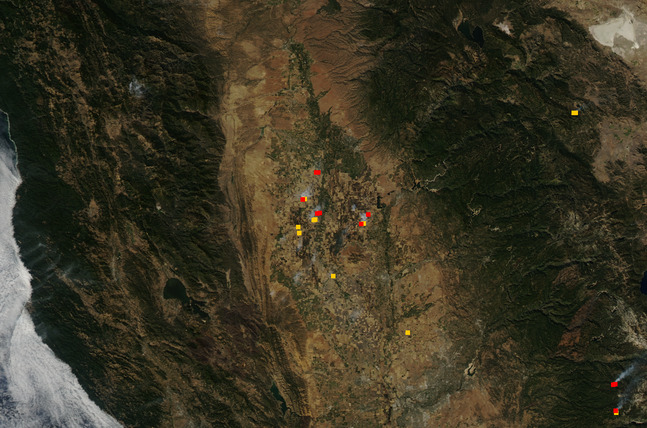
\includegraphics[width=\textwidth]{images/injection/original.jpg}
    \caption{Original image with some fires.}
    \label{fig:injection-orig}
  \end{figure}
\end{frame}

\begin{frame}
  \frametitle{Forest fire detection}
  \framesubtitle{Injecting ficticious fires}

  \begin{figure}
    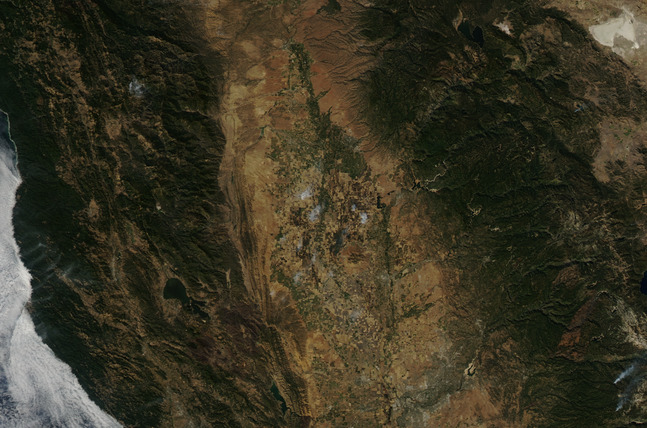
\includegraphics[width=\textwidth]{images/injection/masked_0.jpg}
    \caption{MODIS image with legitimate fires masked out.}
    \label{fig:injection-masked}
  \end{figure}
\end{frame}

\begin{frame}
  \frametitle{Forest fire detection}
  \framesubtitle{Injecting ficticious fires}

  \begin{figure}
    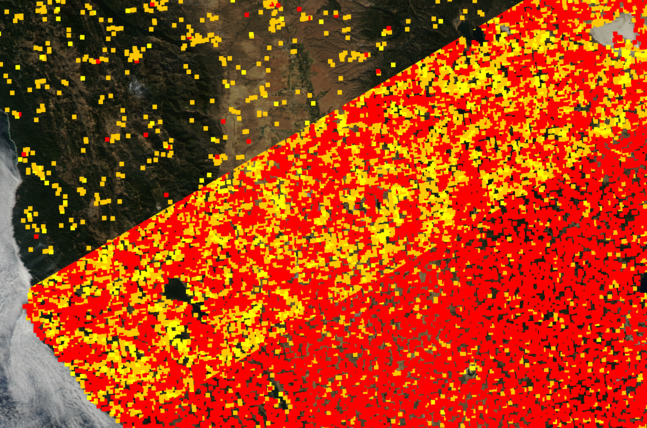
\includegraphics[width=\textwidth]{images/injection/random_combined_diagonal.jpg}
    \caption{Fires randomly injected uniformly across the map.}
    \label{fig:injection-random}
  \end{figure}
\end{frame}

\begin{frame}
  \frametitle{Forest fire detection}
  \framesubtitle{Injecting ficticious fires}

  \begin{figure}
    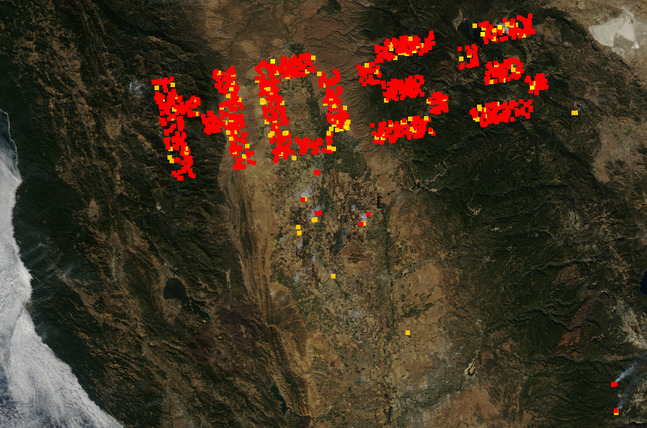
\includegraphics[width=\textwidth]{images/injection/pixels_800_140.jpg}
    \caption{Fine-grained control over the injected fires.}
    \label{fig:injection-location}
  \end{figure}
\end{frame}



\begin{frame}
  \frametitle{Related work}
  Attackers can leverage overshadowing in other domains to manipulate communications and deny service.
  \begin{itemize}[<+->]
    \item Mobile communications -- \textit{Hiding in plain signal: Physical signal overshadowing attack on LTE}~\cite{yang2019hiding}, USENIX 2019
    \item Aircraft -- \textit{Wireless Attacks on Aircraft Instrument Landing Systems}~\cite{sathayeWireless2019}, USENIX 2019
    \item GPS -- \textit{On the requirements for successful GPS spoofing attacks}~\cite{tippenhauer2011requirements}, ACM CCS 2011
    \item EV charging -- \url{https://brokenwire.fail}, K{\"o}hler et. al., University of Oxford
  \end{itemize}
  \note{The idea of overshadowing a signal in this way is not new. There is plenty of existing work in this field.}
\end{frame}

%\begin{frame}[fragile]
%  \frametitle{Related work - US congressional report}
%  \begin{verbatim}
%    This is some quoted text
%  \end{verbatim}
%\end{frame}

\begin{frame}
  \frametitle{Related work - US congressional report}
    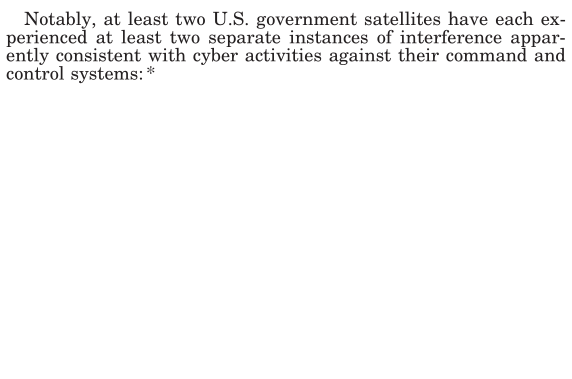
\includegraphics[width=\textwidth]{images/congress_report_1.png}
\end{frame}
\begin{frame}
  \frametitle{Related work - US congressional report}
    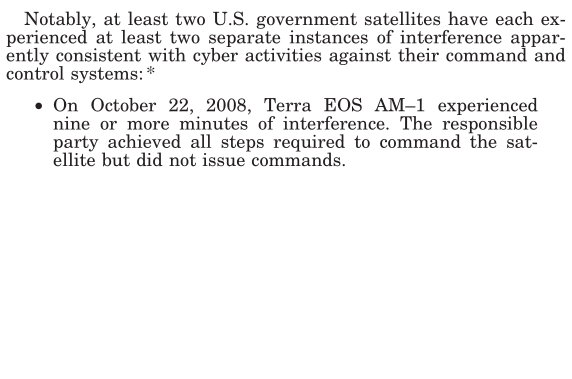
\includegraphics[width=\textwidth]{images/congress_report_2.png}
\end{frame}
\begin{frame}
  \frametitle{Related work - US congressional report}
    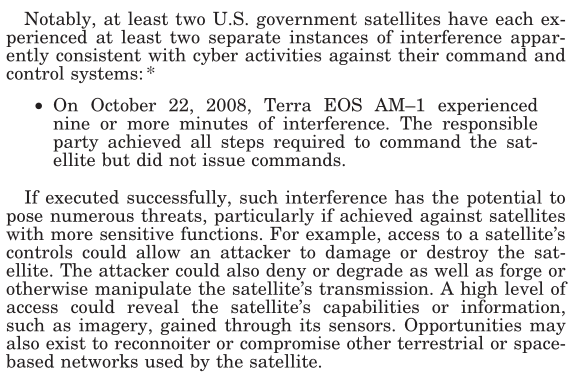
\includegraphics[width=\textwidth]{images/congress_report_3.png}
\end{frame}
\begin{frame}
  \frametitle{Related work - US congressional report}
    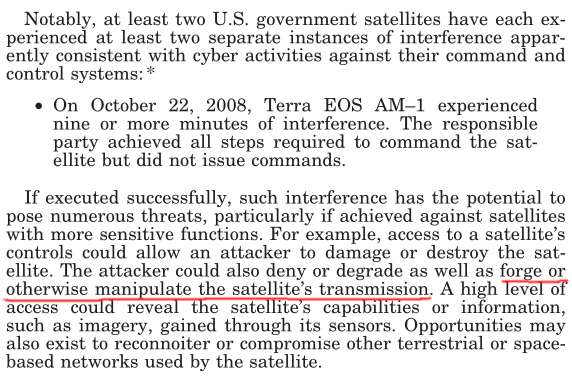
\includegraphics[width=\textwidth]{images/congress_report_4.png}
\end{frame}
\begin{frame}
  \frametitle{Related work - US congressional report}
    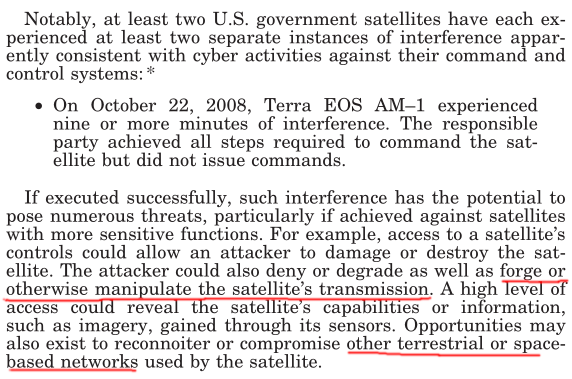
\includegraphics[width=\textwidth]{images/congress_report_5.png}
\end{frame}

\begin{frame}
  \frametitle{This work}
  \framesubtitle{Contributions}
  \begin{itemize}[<+->]
    \item Understand the effect that a modern adversary can have against legacy Earth observing systems
    \item Illustrate the problem with an end-to-end case study, achieving arbitrary image injection and code execution over the processing systems for NASA's FIRMS service
    \item Discuss the impact of other similar attacks against other datasets
    \item Examine the feasibility of the attack through radio simulations
    \item Understand the applicability of existing countermeasures
  \end{itemize}
  \note{In this talk, we'll consider the effect of a modern adversary against NASA's live forest fire detection system, as used in over 160 countries.
  We'll demonstrate end-to-end how overshadowing the physical layer can lead to poisoning the satellite-derived datasets and exploiting the processing systems themselves.
  We demonstrate that an attacker can arbitrarily manipulate fires in the derived dataset to trigger false emergency response or mislead crisis analysis.
  Finally, we demonstrate through radio simulation that it's practical for a ground-based attacker to achieve the required signal injection attack, even against a highly directional dish.
  }
\end{frame}

\begin{frame}
  \frametitle{Threat model}
  \framesubtitle{Adversary's goal}
  Cause disruption to downlink processing systems by emitting counterfeit signals in the vicinity of the receiver, resulting in either:
  \newline

  \begin{itemize}
    \item Affecting the satellite-derived datasets
    \begin{itemize}
      \item Inject false data, disrupting automated detection systems
      \item Mask real data, denying people information
    \end{itemize}
    \item Exploiting or disrupting downlink processing stages
    \begin{itemize}
      \item Achieve denial of service, e.g. by causing pipeline stages to crash
      \item Execute arbitrary core, e.g. by exploiting processing stages that call the shell
    \end{itemize}
  \end{itemize}
\end{frame}

\begin{frame}
  \frametitle{Threat model}
  \framesubtitle{Adversary's capabilities}
  \begin{itemize}
    \item Access to commercially available hardware such as software-defined radios, amplifiers, and antennas.
    \item Can maintain presence in the vicinity of a receiver.
    \item Is ground based, so cannot emit signals directly within the beam of the receiver.
  \end{itemize}
\end{frame}

\begin{frame}
  \frametitle{Threat model}
  \framesubtitle{Estimated cost}

  \begin{figure}
      \centering
      \begin{tabular}{ l | l }
        \textbf{Hardware component} & \textbf{Cost} \\
        \hline
        limeSDR & $598$ USD \\
        X-Band transmitter & $22,800$ EUR \\
        Compatible antenna & $6,400$ EUR \\
        \hline
        Total & \~{}$30,000$ EUR
      \end{tabular}
      \label{tab:cost}
  \end{figure}

  Within the budget of a motivated hobbyist.

  The limitations of this setup are explored through the radio simulations later.
\end{frame}

% Our attack is different because we achieve the same effects without requiring satellite control compromise

% BrokenWire (presentation from before)
% Aqua uplink
% However, no existing work has shown the effects on the downlink receiver software

% TODO: case study: GPS
% At end: case study on how GPS encryption can be circumvented


\begin{frame}
  \frametitle{Satellite downlink communications}
  \begin{figure}
  \centering
      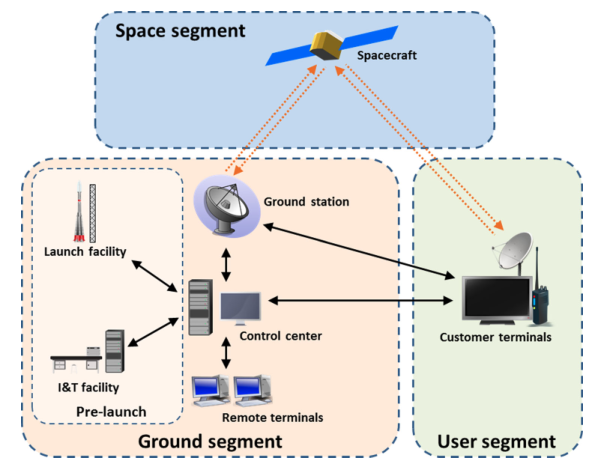
\includegraphics[width=0.7\textwidth]{images/space_segment.png}
      \caption{Typical satellite mission control architecture}
      \label{fig:space_segment}
  \end{figure}
\end{frame}
% In a common satellite mission, there are three segments

\begin{frame}
  \frametitle{Case study 1: dataset poisoning}
  \framesubtitle{Attack steps}
  We consider as a case study the FIRMS system derived from Aqua
  
  \begin{itemize}[<+->]
    \item Obtain/capture legitimate data
    \begin{itemize}
      \item Download from NASA distributed data archive
    \end{itemize}

    \item Process it to add/remove artefacts
    \begin{itemize}
      \item Reverse engineer the image format, and write an image manipulation program
    \end{itemize}

    \item Reformat it into raw samples
    \begin{itemize}
      \item Implement the data link protocol encoder and generate the raw data frames
    \end{itemize}

    \item Overshadow with a software-defined radio
    \begin{itemize}
      \item QPSK modulate the data onto the X-band in the vicinity of the receiver
    \end{itemize}
  \end{itemize}
\end{frame}


\begin{frame}
  \frametitle{Case study 2: exploit downlink processing stages}
  \framesubtitle{Attack steps}
  \begin{itemize}[<+->]
   \item Obtain downlink decoder software and perform security audit
   \begin{itemize}
     \item Look for possible exploits around manual memory management and execution boundaries
   \end{itemize}

    \item Construct payload packet to trigger vulnerability chain
    \begin{itemize}
      \item Violate assumptions about the protocol headers
    \end{itemize}

    \item Reformat it into raw samples
    \begin{itemize}
      \item Implement the data link protocol encoder and generate the raw data frames
    \end{itemize}

    \item Overshadow with a software-defined radio
    \begin{itemize}
      \item QPSK modulate the data onto the X-band in the vicinity of the receiver
    \end{itemize}
  \end{itemize}
\end{frame}


\begin{frame}
  \frametitle{Case study 1: dataset poisoning}
  \framesubtitle{Data capture}
  \begin{itemize}[<+->]
    \item Derived datasets from Aqua available from distributed web archives from NASA's website
    \item Can be found at multiple stages of processing
    \item The files are separated according to a timestamp format, so the attacker needs to find an image of the desired location by using the satellite's orbital parameters
  \end{itemize}
  
  \url{https://ladsweb.modaps.eosdis.nasa.gov}

\note{
  LADSWeb archive - can download datasets at several different levels of processing
  We want the lowest form possible
  To know what to download, we need to do some reversing of the satellite coordinates and timestamp etc
  Can theoretically do this in the live setting as well
}
\end{frame}

% TODO: add into here the format for names of the data
\begin{frame}
  \frametitle{Case study 1: dataset poisoning}
  \framesubtitle{Data capture}
  \begin{figure}
    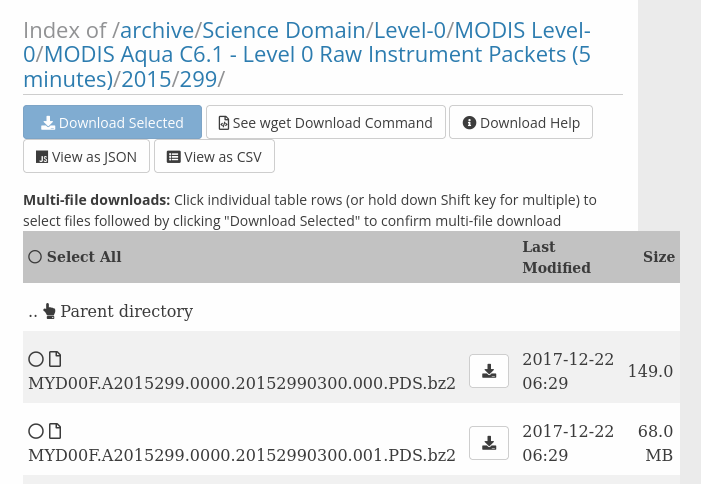
\includegraphics[width=0.8\textwidth]{images/level0.png}
    \caption{LAADS DAAC archive centre download}
    \label{fig:level0}
  \end{figure}  
  \url{https://ladsweb.modaps.eosdis.nasa.gov/archive/Science\%20Domain/Level-0/MODIS\%20Level-0/MODIS\%20Aqua\%20C6.1\%20-\%20Level\%200\%20Raw\%20Instrument\%20Packets\%20(5\%20minutes)/2015/299/}

\end{frame}

\begin{frame}
  \frametitle{Case study 1: dataset poisoning}
  \framesubtitle{Data processing: image format reversing}
  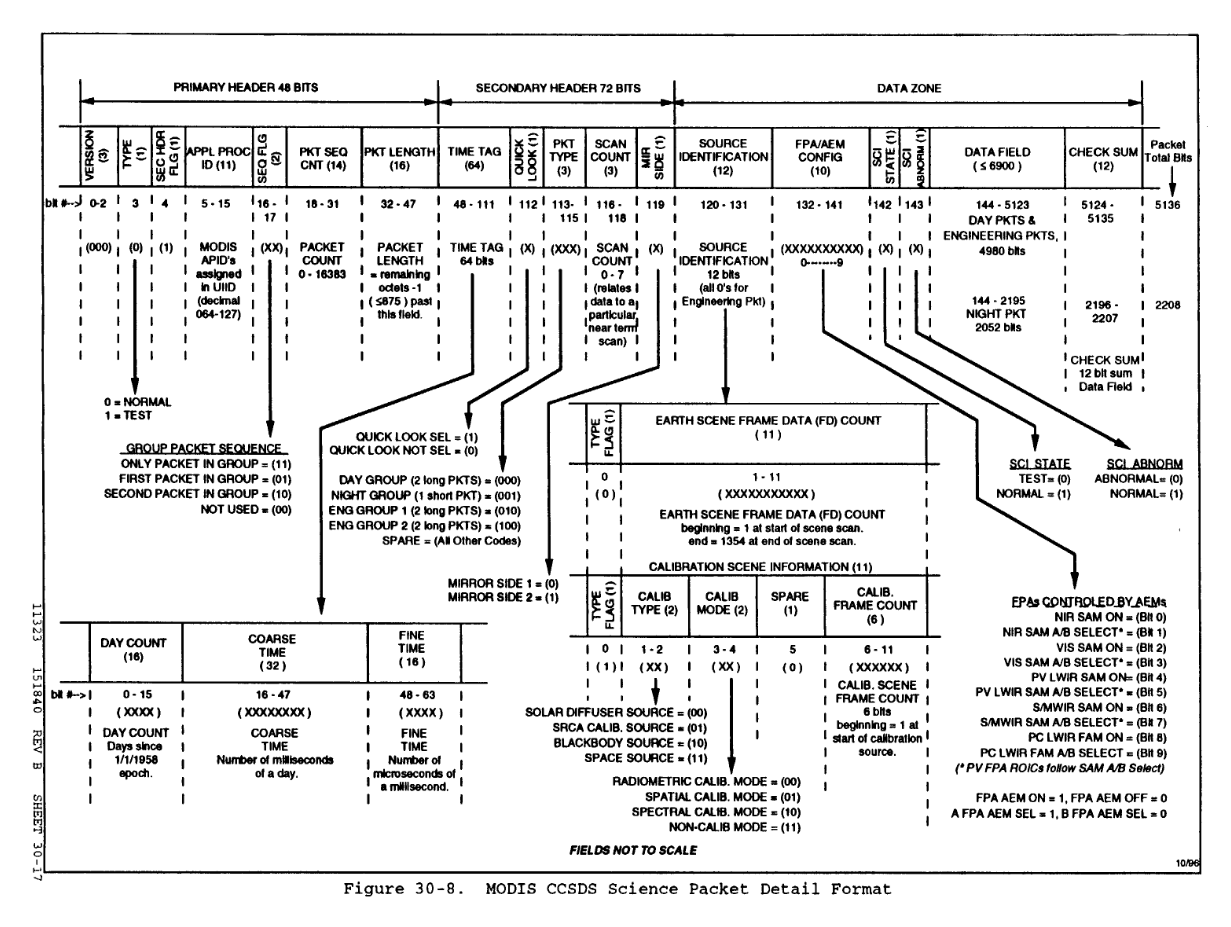
\includegraphics[width=\textwidth]{images/image_format.png}

  \note{We must firstly reverse engineer the image format}
\end{frame}

\begin{frame}
  \frametitle{Case study 1: dataset poisoning}
  \framesubtitle{Data processing: encoding/decoding}

  We write a library to support encoding/decoding this image format
\end{frame}


\begin{frame}
  \frametitle{Case study 1: dataset poisoning}
  \framesubtitle{Reformatting: CCSDS protocols}
  \centering
  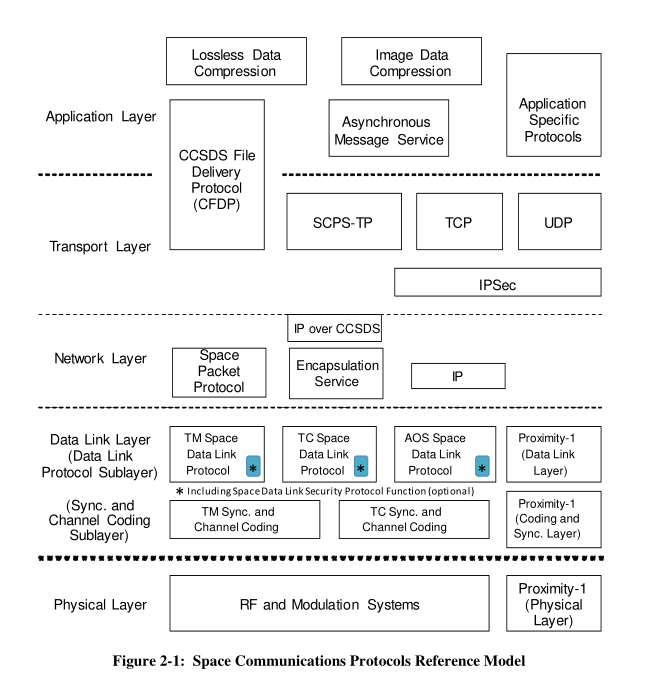
\includegraphics[width=0.65\textwidth]{images/protocols.png}
\end{frame}

\begin{frame}
  \frametitle{Case study 1: dataset poisoning}
  \framesubtitle{Reformatting: Aqua's protocols}
  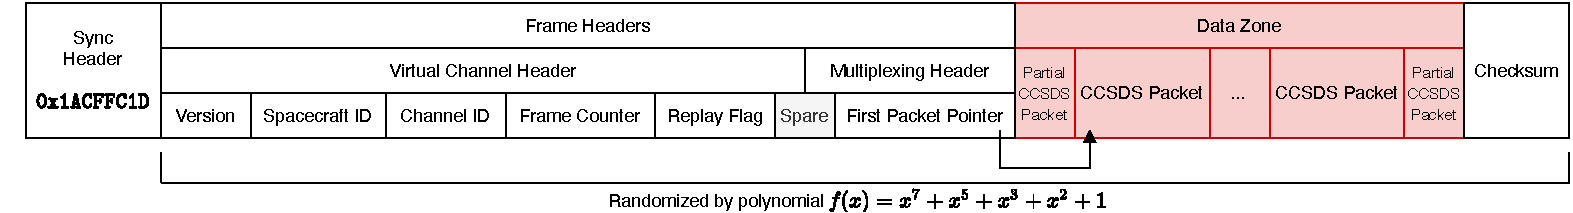
\includegraphics[width=\textwidth]{images/cadu_diagram.pdf}
\end{frame}

\begin{frame}
  \frametitle{Case study 1: dataset poisoning}
  \framesubtitle{Reformatting}
  \begin{itemize}
    \item Aqua uses a non-standardised data link level protocol
    \item This encapsulates the standardised space packet protocol used at the network layer
  \end{itemize}

  We write a library to support encoding/decoding the network and data link layers
\end{frame}
% We set up a rolled-your-own data link level protocol so that later we can talk about exploiting it
\begin{frame}
  \frametitle{Case study 1: dataset poisoning}
  \framesubtitle{Example}
  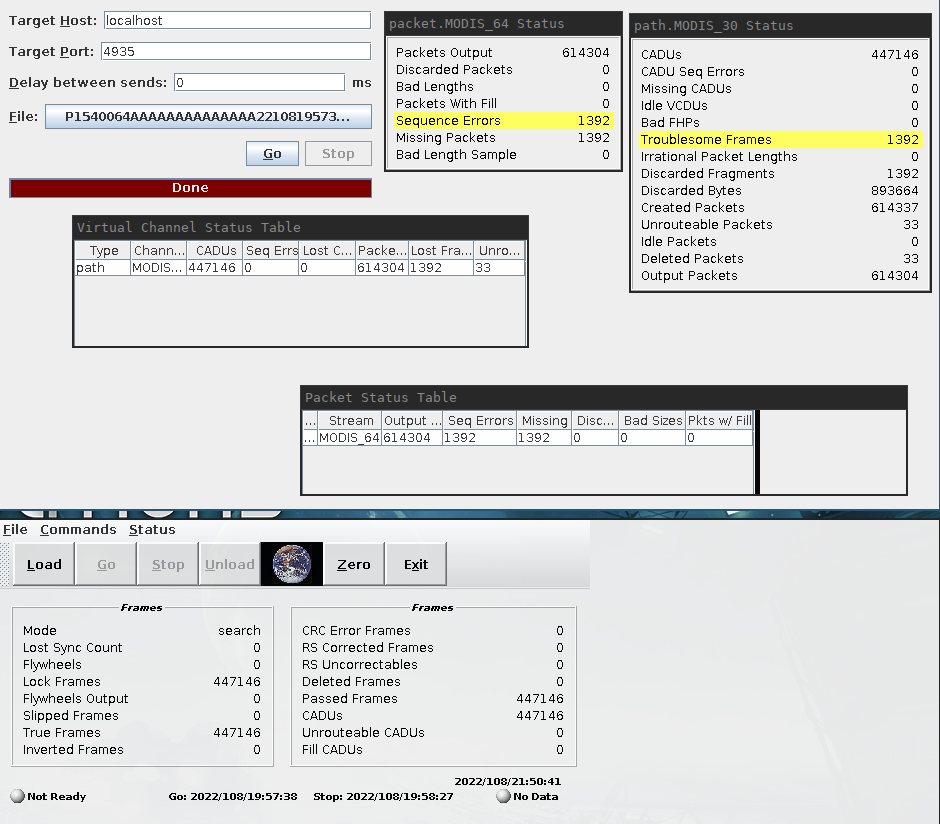
\includegraphics[width=0.7\textwidth]{images/rtstps_incorrect.png}
\end{frame}

\begin{frame}
  \frametitle{Case study 1: dataset poisoning}
  \framesubtitle{Example}
  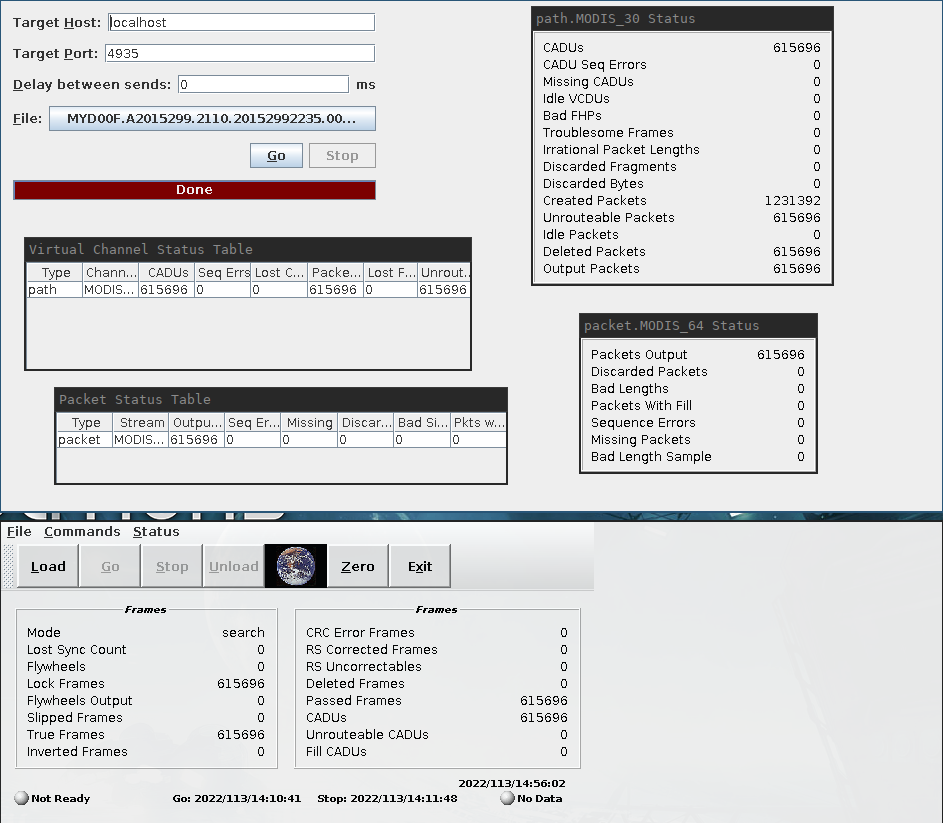
\includegraphics[width=0.7\textwidth]{images/rtstps_correct.png}
\end{frame}

\begin{frame}
  \frametitle{Forest fire detection}
  \framesubtitle{Injecting ficticious fires}

  \begin{figure}
    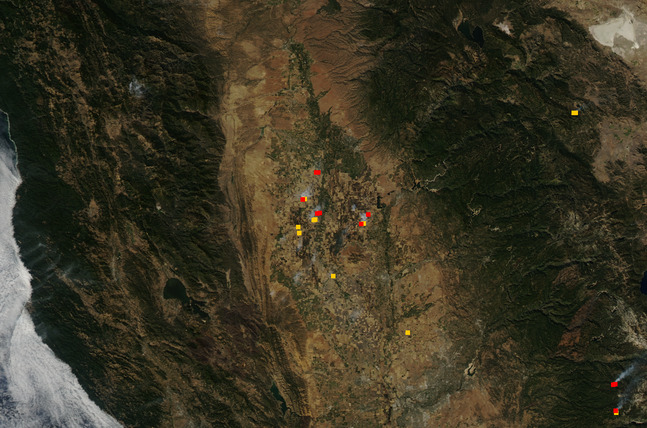
\includegraphics[width=\textwidth]{images/injection/original.jpg}
    \caption{Original image with some fires.}
    \label{fig:injection-orig}
  \end{figure}
\end{frame}

\begin{frame}
  \frametitle{Forest fire detection}
  \framesubtitle{Injecting ficticious fires}

  \begin{figure}
    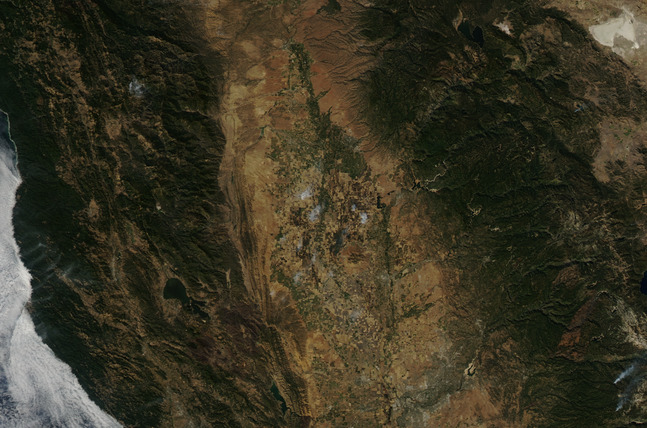
\includegraphics[width=\textwidth]{images/injection/masked_0.jpg}
    \caption{MODIS image with legitimate fires masked out.}
    \label{fig:injection-masked}
  \end{figure}
\end{frame}

\begin{frame}
  \frametitle{Case study 2: exploit downlink processing stages}
  \framesubtitle{Attack steps}
  \begin{itemize}
   \item Obtain downlink decoder software and perform security audit
   \begin{itemize}
     \item Look for possible exploits around manual memory management and execution boundaries
   \end{itemize}

    \item Construct payload packet to trigger vulnerability chain
    \begin{itemize}
      \item Violate assumptions about the protocol headers
    \end{itemize}

    \item Reformat it into raw samples
    \begin{itemize}
      \item Implement the data link protocol encoder and generate the raw data frames
    \end{itemize}

    \item Overshadow with a software-defined radio
    \begin{itemize}
      \item QPSK modulate the data onto the X-band in the vicinity of the receiver
    \end{itemize}
  \end{itemize}
\end{frame}

\begin{frame}
  \frametitle{Case study 2: exploit downlink processing stages}
  \framesubtitle{Obtain downlink decoder software}
  With a research account, anyone can download the entire set of decoding software from NASA's \textit{Direct Readout Laboratory}
  \url{https://directreadout.sci.gsfc.nasa.gov/}
\end{frame}

\begin{frame}
  \frametitle{Case study 2: exploit downlink processing stages}
  \framesubtitle{Create decoding simulated environment}
  \centering
  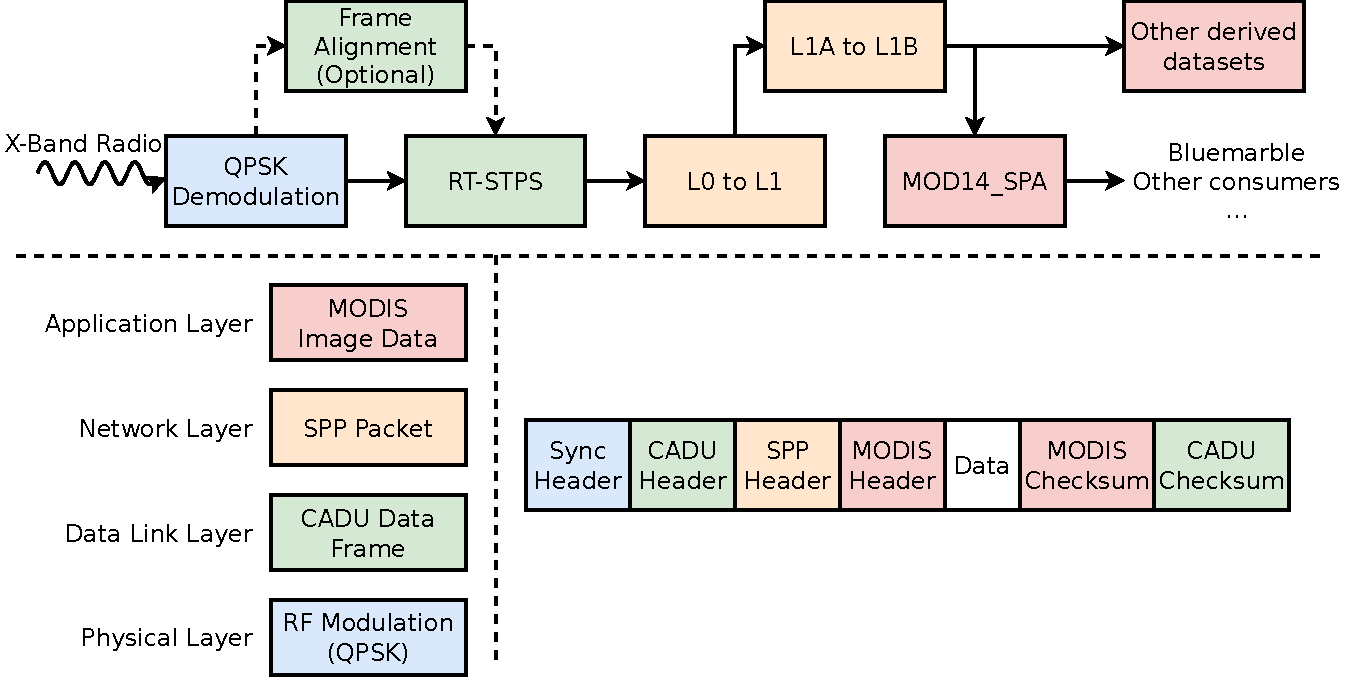
\includegraphics[width=0.8\textwidth]{images/attack_types.pdf}
  \url{https://github.com/ssloxford/firefly/tree/master/decoder_pipeline}
\end{frame}

\begin{frame}
  \frametitle{Case study 2: exploit downlink processing stages}
  \framesubtitle{Reformatting: Aqua's protocols}
  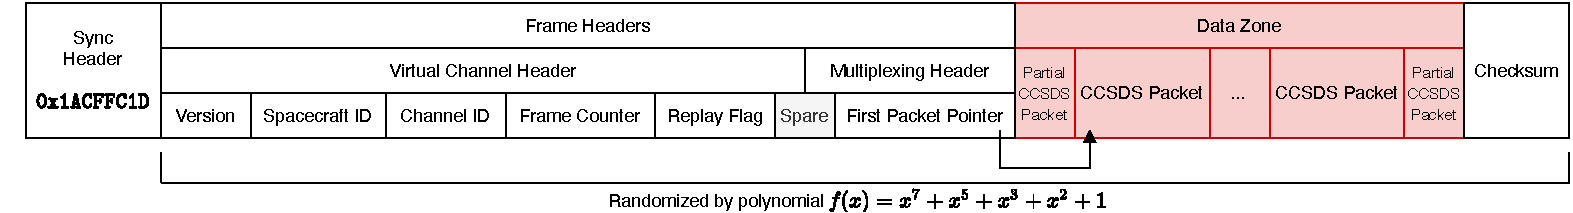
\includegraphics[width=\textwidth]{images/cadu_diagram.pdf}
  \note{Number of causes of concern: L0 to L1 made of many disparate components, interacting across boundaries with access to the shell. Using C programs that don't pay huge attention to managing memory correctly, and using a slightly buggy protocol header parser.}
\end{frame}

\begin{frame}
  \frametitle{Case study 2: exploit downlink processing stages}
  \framesubtitle{Analyse software for exploits}

  \begin{itemize}[<+->]
    \item Usual problems with legacy software here, and we find a kill chain!
    \item What if we just make the header pointer point past the end of the packet?
    \item The NASA software catches this case, but it might not
  \end{itemize}
\end{frame}

\begin{frame}
  \frametitle{Case study 2: exploit downlink processing stages}
  \framesubtitle{Construct a payload}
  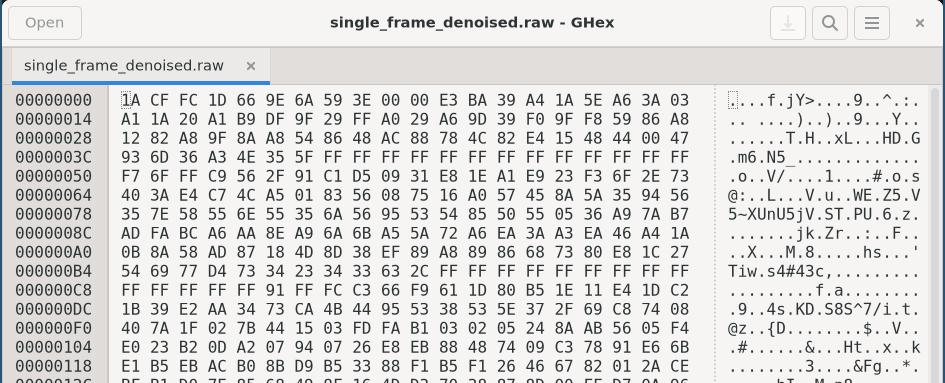
\includegraphics[width=\textwidth]{images/hex.png}

  We use a hex editor to manipulate the bytes, and some tools from our packet manipulation repo.
\end{frame}

\begin{frame}
  \frametitle{Evaluation: overall attack}
  \begin{figure}
      \centering
      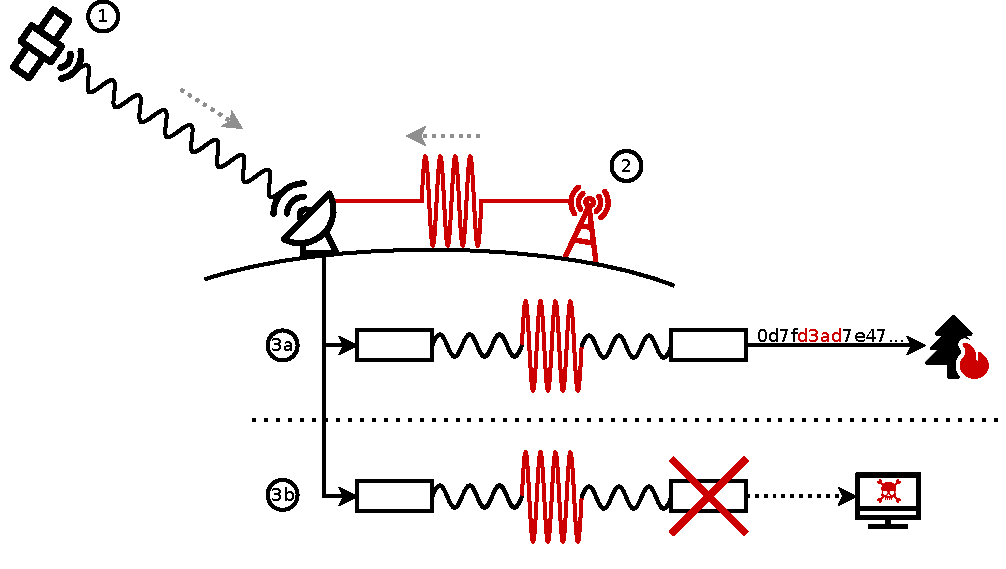
\includegraphics[width=0.7\textwidth]{images/attack_illustration.pdf}
      \label{fig:attack-illustration}
  \end{figure}
  So far, we've generated the signal for the attacker to emit.

  To evaluate this strategy in practise, we need to know the radio requirements for a successful injection.
\end{frame}

\begin{frame}
  \frametitle{Evaluation}
  To evaluate, we ...
  \begin{itemize}[<+->]
    \item Set up a radio pipeline to closely mimic the effects of a ground-based attacker
    \item Measure how antenna strength and distance affect the bit error rate at the decoder
    \item Calculate bounds by considering the corrective ability of the checksum
  \end{itemize}
\end{frame}

\begin{frame}
  \frametitle{Evaluation}
  \framesubtitle{Experimental setup}
  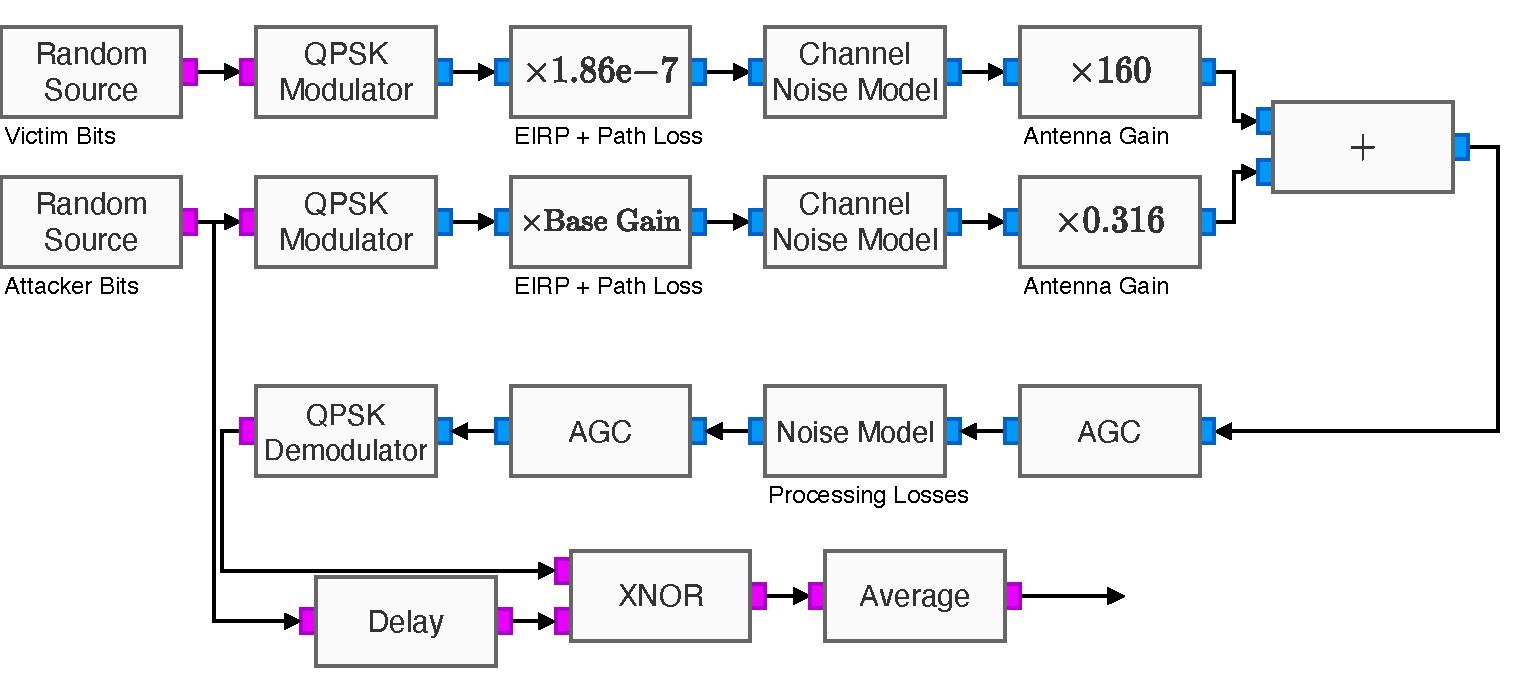
\includegraphics[width=\textwidth]{images/overshadowing_pipeline.pdf}
\end{frame}

\begin{frame}
  \frametitle{Evaluation}
  \framesubtitle{Results}
  \begin{figure}
      \centering
      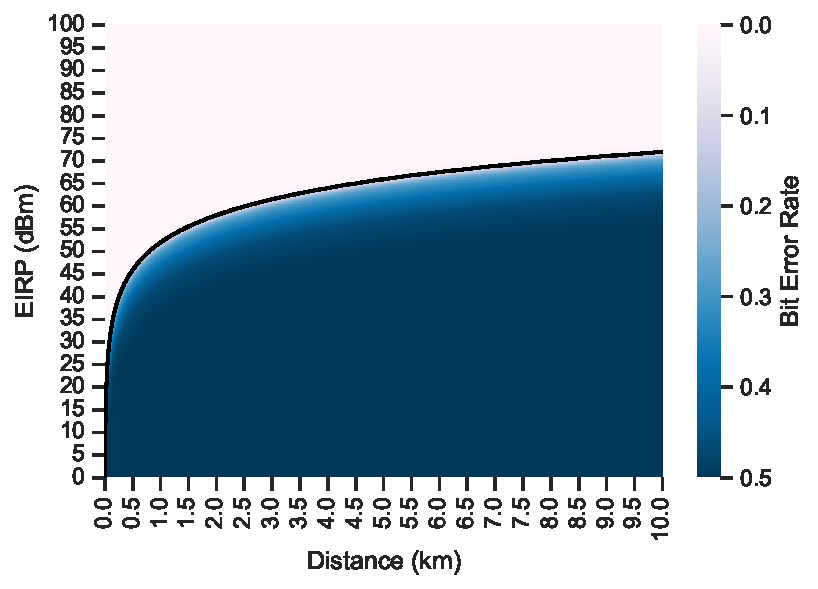
\includegraphics[width=0.6\columnwidth]{images/distance_eirp_heatmap_95.pdf}
      \caption{The bit error rate of the injected signal as the attacker varies EIRP and distance from the receiver. The values beyond which the bit error rate drops below $5$\% are indicated using a line.}
      \label{fig:distance_eirp}
  \end{figure}
  Our transmitter has EIRP (Effective Isotropic Radiated Power) of 49dBm.
\end{frame}

\begin{frame}
  \frametitle{Evaluation}
  \framesubtitle{Results}
  \begin{figure}
      \centering
      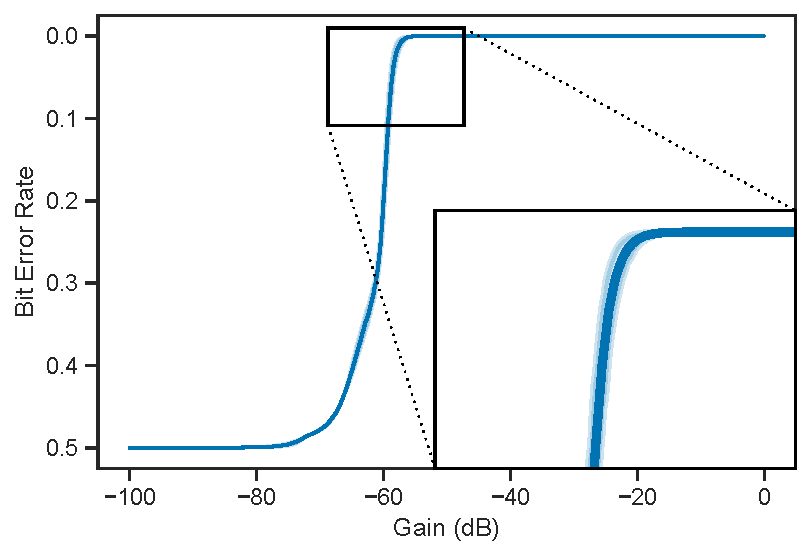
\includegraphics[width=0.7\columnwidth]{images/overshadowing_ber_2.pdf}
      \caption{Error rate of attacker-injected bits as the signal strength at the receiver increases. The small shaded region represents the range of values under different levels of background and system noise.}
      \label{fig:overshadowing_ber}
  \end{figure}
\end{frame}

\begin{frame}
  \frametitle{Discussion}
  \begin{itemize}
    \item A sufficiently motivated adversary can successfully pull off signal injection attacks
    \item These attacks can result in dataset poisoning and exploiting the decoding software
    \item Other similarly decryptable satellite systems may be vulnerable to similar techniques
  \end{itemize}
\end{frame}

\begin{frame}
  \frametitle{Countermeasures}
  \framesubtitle{Cryptographic solutions}
  \begin{itemize}
    \item Gives strong guarantees of data integrity, authenticity, non-repudiation, etc.
    \item Satellites have long lifespans, so currently secure crypto might become breakable (post-quantum)
    \item Retrofitting crypto onto existing satellite systems is infeasible
  \end{itemize}
\end{frame}

\begin{frame}
  \frametitle{Countermeasures}
  \framesubtitle{Timing analysis}
  \begin{itemize}
    \item Multiple receiver triangulation to determine attacker location
    \item Requires coordination between multiple groundstations
  \end{itemize}
\end{frame}

\begin{frame}
  \frametitle{Countermeasures}
  \framesubtitle{Waveform analysis}
  \begin{itemize}
    \item Looking at properties of the legitimate/overshadowed signal
    \item Traditional approaches like analysing signal-to-noise may prove effective
    \item New ML approaches starting to be created (PAST-AI)
  \end{itemize}
\end{frame}

\begin{frame}
  \frametitle{Countermeasures}
  \framesubtitle{Data inspection}
  \begin{itemize}
    \item Look for artefacts of tampering in the packets, and compare packets from multiple groundstations
    \item Doesn't require any hardware modifications to the receiver
    \item Protects against decoder exploitation
    \item Doesn't protect against dataset poisoning
  \end{itemize}
\end{frame}

\begin{frame}
  \frametitle{Conclusion}
  \begin{itemize}[<+->]
    \item Signal injection against satellite downlinks are currently effective against decryptable classes of satellites
    \item Through an end-to-end case study, we demonstrated that the EOS satellites are vulnerable, with wide ramifications
    \item Only a moderate equipment budget is required to perform these attacks
    \item Currently proposed countermeasures would increase the complexity of performing this attack in practice
    \item Future work should consider a comprehensive overview of similarly vulnerable systems
  \end{itemize}
\end{frame}

% TODO: end card with socials, contact details, etc.


\begin{frame}
  \frametitle{Citations}
  \bibliographystyle{IEEEtranS}
  \bibliography{IEEEabrv,refs}
\end{frame}

\end{document}
